\documentclass[xcolor=dvipsnames]{beamer}\usepackage{graphicx, color}
%% maxwidth is the original width if it is less than linewidth
%% otherwise use linewidth (to make sure the graphics do not exceed the margin)
\makeatletter
\def\maxwidth{ %
  \ifdim\Gin@nat@width>\linewidth
    \linewidth
  \else
    \Gin@nat@width
  \fi
}
\makeatother

\definecolor{fgcolor}{rgb}{0.2, 0.2, 0.2}
\newcommand{\hlnumber}[1]{\textcolor[rgb]{0,0,0}{#1}}%
\newcommand{\hlfunctioncall}[1]{\textcolor[rgb]{0.501960784313725,0,0.329411764705882}{\textbf{#1}}}%
\newcommand{\hlstring}[1]{\textcolor[rgb]{0.6,0.6,1}{#1}}%
\newcommand{\hlkeyword}[1]{\textcolor[rgb]{0,0,0}{\textbf{#1}}}%
\newcommand{\hlargument}[1]{\textcolor[rgb]{0.690196078431373,0.250980392156863,0.0196078431372549}{#1}}%
\newcommand{\hlcomment}[1]{\textcolor[rgb]{0.180392156862745,0.6,0.341176470588235}{#1}}%
\newcommand{\hlroxygencomment}[1]{\textcolor[rgb]{0.43921568627451,0.47843137254902,0.701960784313725}{#1}}%
\newcommand{\hlformalargs}[1]{\textcolor[rgb]{0.690196078431373,0.250980392156863,0.0196078431372549}{#1}}%
\newcommand{\hleqformalargs}[1]{\textcolor[rgb]{0.690196078431373,0.250980392156863,0.0196078431372549}{#1}}%
\newcommand{\hlassignement}[1]{\textcolor[rgb]{0,0,0}{\textbf{#1}}}%
\newcommand{\hlpackage}[1]{\textcolor[rgb]{0.588235294117647,0.709803921568627,0.145098039215686}{#1}}%
\newcommand{\hlslot}[1]{\textit{#1}}%
\newcommand{\hlsymbol}[1]{\textcolor[rgb]{0,0,0}{#1}}%
\newcommand{\hlprompt}[1]{\textcolor[rgb]{0.2,0.2,0.2}{#1}}%

\usepackage{framed}
\makeatletter
\newenvironment{kframe}{%
 \def\at@end@of@kframe{}%
 \ifinner\ifhmode%
  \def\at@end@of@kframe{\end{minipage}}%
  \begin{minipage}{\columnwidth}%
 \fi\fi%
 \def\FrameCommand##1{\hskip\@totalleftmargin \hskip-\fboxsep
 \colorbox{shadecolor}{##1}\hskip-\fboxsep
     % There is no \\@totalrightmargin, so:
     \hskip-\linewidth \hskip-\@totalleftmargin \hskip\columnwidth}%
 \MakeFramed {\advance\hsize-\width
   \@totalleftmargin\z@ \linewidth\hsize
   \@setminipage}}%
 {\par\unskip\endMakeFramed%
 \at@end@of@kframe}
\makeatother

\definecolor{shadecolor}{rgb}{.97, .97, .97}
\definecolor{messagecolor}{rgb}{0, 0, 0}
\definecolor{warningcolor}{rgb}{1, 0, 1}
\definecolor{errorcolor}{rgb}{1, 0, 0}
\newenvironment{knitrout}{}{} % an empty environment to be redefined in TeX

\usepackage{alltt}
%%\usepackage[dvipsnames]{xcolor}

\usefonttheme[onlymath]{serif}

\setbeamercolor{title}{fg=black}
\setbeamercolor{frametitle}{fg=black}

\setbeamertemplate{itemize items}[circle] 
\setbeamercolor{itemize item}{fg=black}
\IfFileExists{upquote.sty}{\usepackage{upquote}}{} 
\begin{document}

\title{Reserving, linear regression, MRMR and R}
\author{Brian A. Fannin}

\maketitle

% very important to use option [fragile] for frames containing code output!




\begin{frame} {Agenda}
  \begin{itemize}
    \item Introducing MRMR
    \item Data visualization 
    \item Linear modeling
    \item Fit diagnostics
    \item Projection
    \item Grouped visualization
    \item Another view of regression
    \item Further
  \end{itemize}
\end{frame}

\begin{frame} {Introducing MRMR}
  MRMR is another R package for use in analyzing reserves.
  
  MRMR was heavily influenced by the following:
  \begin{itemize}
    \item Andrew Gelman and Jennifer Hill, "Data Analysis Using Regression and Multilevel/Hierarchical Models"
    \item ggplot2 and Hadley Wickham
    \item Leigh Halliwell and Judge et al
  \end{itemize}
\end{frame}

\begin{frame} {MRMR Structure}
  MRMR supports three S4 classes: Triangle, TriangleModel and TriangleProjection. These have a rough correspondence to the behavior of functions lm, glm and lme4.
  
  \begin{tabular} { | l | l | l | }
    \hline
    Item & R & MRMR \\ \hline
    Data storage & Data frame & Triangle \\ \hline
    Model & Function lm (S3 object) & TriangleModel \\ \hline
    Project & Function predict (vector) & TriangleProjection \\ 
    \hline
  \end{tabular}
\end{frame}

\begin{frame}[fragile]{Startup MRMR}
\begin{knitrout}
\definecolor{shadecolor}{rgb}{0.969, 0.969, 0.969}\color{fgcolor}\begin{kframe}
\begin{alltt}
\hlfunctioncall{library}(MRMR)
`?`(MRMR)
\end{alltt}
\end{kframe}
\end{knitrout}

\end{frame}

\begin{frame}{Basic requirements}
  A triangle object must possess the following data elements:
  \begin{itemize}
    \item Temporal dimensions for origin period, development lag and evaluation date. These are stored as lubridate objects.
    \item Measures
      \begin{itemize}
        \item Stochastic - Loss, claim, etc. These are time series variables and candidates for prediction. MRMR will adjust these so that incremental, cumulative and prior cumulative columns are formed.
        \item Static - Typically exposure variables. These will not be adjusted
      \end{itemize}
    \item One or more grouping elements
  \end{itemize}
\end{frame}

\begin{frame}[fragile]{lubridate}
\begin{knitrout}
\definecolor{shadecolor}{rgb}{0.969, 0.969, 0.969}\color{fgcolor}\begin{kframe}
\begin{alltt}
myPeriod = \hlfunctioncall{months}(6)
myPeriod/\hlfunctioncall{months}(1)
\end{alltt}


{\ttfamily\noindent\itshape\color{messagecolor}{\#\# estimate only: convert to intervals for accuracy}}\begin{verbatim}
## [1] 6
\end{verbatim}
\begin{alltt}
\hlfunctioncall{mdy}(\hlstring{"06-30-2012"})
\end{alltt}
\begin{verbatim}
## [1] "2012-06-30 UTC"
\end{verbatim}
\begin{alltt}
\hlfunctioncall{typeof}(\hlfunctioncall{mdy}(\hlstring{"06-30-2012"}))
\end{alltt}
\begin{verbatim}
## [1] "double"
\end{verbatim}
\end{kframe}
\end{knitrout}

\end{frame}

\begin{frame}[fragile]{A very basic example}
\begin{knitrout}
\definecolor{shadecolor}{rgb}{0.969, 0.969, 0.969}\color{fgcolor}\begin{kframe}
\begin{alltt}
AccidentYear = \hlfunctioncall{c}(2002, 2002, 2002, 2003, 
    2003, 2004)

Month = \hlfunctioncall{c}(12, 24, 36, 12, 24, 12)

Paid = \hlfunctioncall{c}(2318, 7932, 13822, 1743, 6240, 2221)

EP = \hlfunctioncall{c}(61183, 61183, 61183, 69175, 69175, 
    99322)

df = \hlfunctioncall{data.frame}(AccidentYear = AccidentYear, 
    Month = Month, Paid = Paid, EP = EP)
\hlfunctioncall{head}(df)
\end{alltt}
\end{kframe}
\end{knitrout}

\end{frame}

\begin{frame}[fragile] {Moving the data into a Triangle object}
\begin{knitrout}
\definecolor{shadecolor}{rgb}{0.969, 0.969, 0.969}\color{fgcolor}\begin{kframe}
\begin{alltt}
myTriangle = \hlfunctioncall{newTriangle}(TriangleData = df, 
    OriginPeriods = AccidentYear, DevelopmentLags = Month, 
    Cumulative = TRUE, StochasticMeasures = \hlfunctioncall{c}(\hlstring{"Paid"}), 
    StaticMeasures = \hlfunctioncall{c}(\hlstring{"EP"}), Verbose = FALSE)
\end{alltt}
\end{kframe}
\end{knitrout}

\end{frame}

\begin{frame}[fragile]{What's in a Triangle object?}
\begin{knitrout}
\definecolor{shadecolor}{rgb}{0.969, 0.969, 0.969}\color{fgcolor}\begin{kframe}
\begin{alltt}
\hlfunctioncall{slotNames}(myTriangle)
\end{alltt}
\begin{verbatim}
## [1] "TriangleData"       
## [2] "TriangleName"       
## [3] "OriginPeriodType"   
## [4] "DevelopmentInterval"
## [5] "StaticMeasures"     
## [6] "StochasticMeasures" 
## [7] "Groups"
\end{verbatim}
\end{kframe}
\end{knitrout}

\end{frame}

\begin{frame}[fragile]{What sort of data frame have I created?}
\begin{knitrout}
\definecolor{shadecolor}{rgb}{0.969, 0.969, 0.969}\color{fgcolor}\begin{kframe}
\begin{alltt}
\hlfunctioncall{names}(myTriangle@TriangleData)
\end{alltt}
\begin{verbatim}
##  [1] "OriginPeriod"       
##  [2] "DevelopmentLag"     
##  [3] "EvaluationDate"     
##  [4] "DevInteger"         
##  [5] "OriginPeriodStart"  
##  [6] "OriginPeriodEnd"    
##  [7] "CalendarPeriodStart"
##  [8] "CalendarPeriodEnd"  
##  [9] "CalendarPeriod"     
## [10] "Group"              
## [11] "EP"                 
## [12] "CumulativePaid"     
## [13] "IncrementalPaid"    
## [14] "PriorPaid"
\end{verbatim}
\end{kframe}
\end{knitrout}

\end{frame}

\begin{frame}[fragile]{A very basic plot}
\begin{knitrout}
\definecolor{shadecolor}{rgb}{0.969, 0.969, 0.969}\color{fgcolor}\begin{kframe}
\begin{alltt}
\hlfunctioncall{plotTriangle}(myTriangle, Predictor = \hlstring{"DevInteger"}, 
    Response = \hlstring{"CumulativePaid"})
\end{alltt}
\end{kframe}
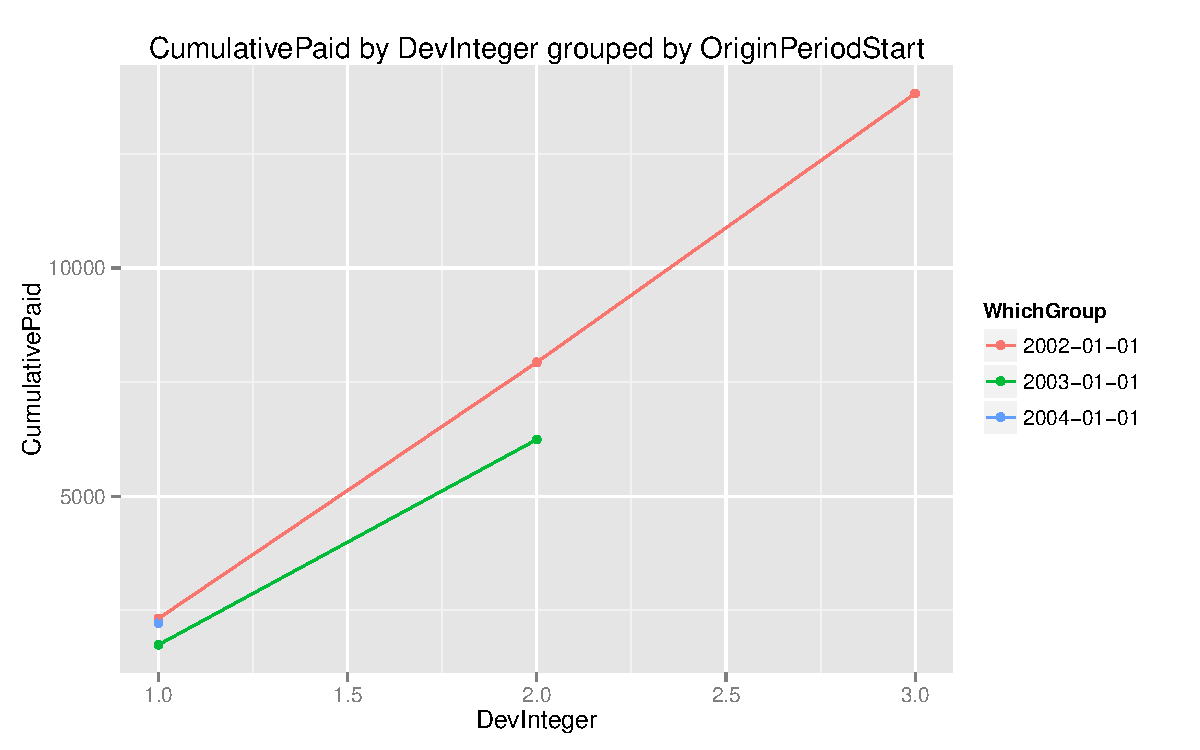
\includegraphics[width=\maxwidth]{figure/VeryBasicExample4} 

\end{knitrout}

\end{frame}

\begin{frame}[fragile]{Something more complex}
\begin{knitrout}
\definecolor{shadecolor}{rgb}{0.969, 0.969, 0.969}\color{fgcolor}\begin{kframe}
\begin{alltt}
\hlfunctioncall{data}(Friedland)
\hlfunctioncall{plotTriangle}(Friedland, Predictor = \hlstring{"DevInteger"}, 
    Response = \hlstring{"CumulativePaid"})
\end{alltt}
\end{kframe}
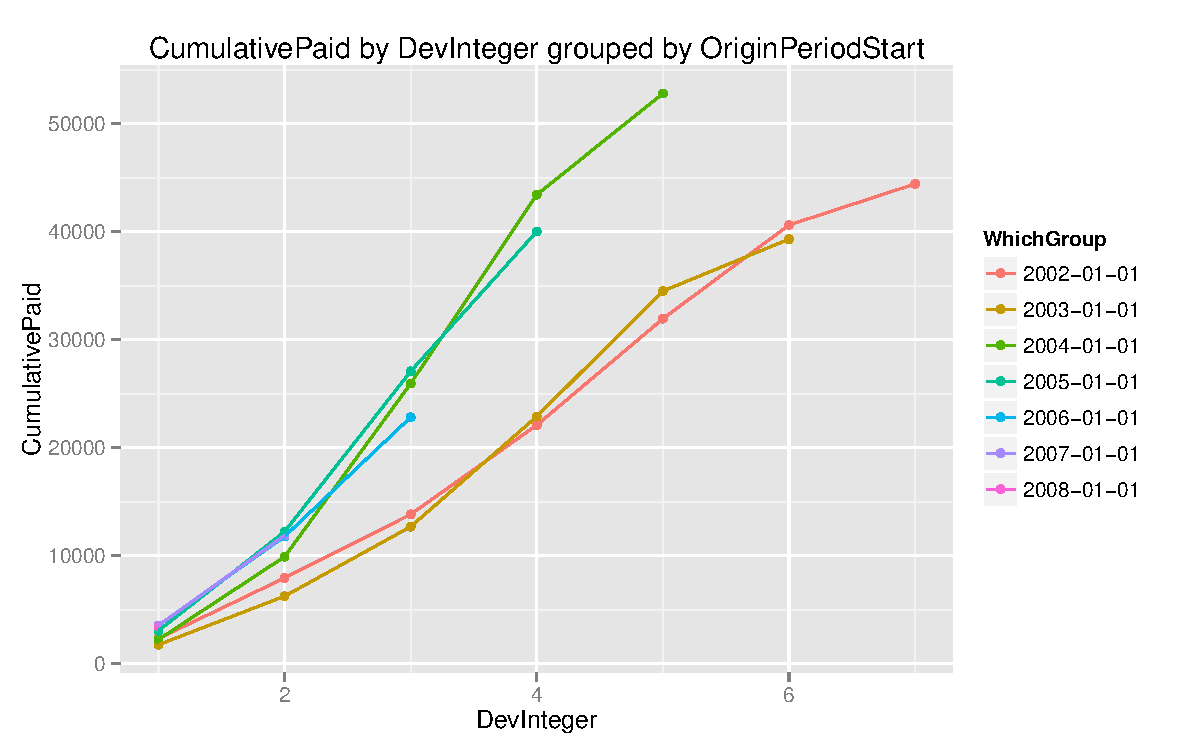
\includegraphics[width=\maxwidth]{figure/Friedland1} 

\end{knitrout}

\end{frame}

\begin{frame}[fragile]{Change the response term}
\begin{knitrout}
\definecolor{shadecolor}{rgb}{0.969, 0.969, 0.969}\color{fgcolor}\begin{kframe}
\begin{alltt}
\hlfunctioncall{plotTriangle}(Friedland, Predictor = \hlstring{"DevInteger"}, 
    Response = \hlstring{"IncrementalPaid"})
\end{alltt}
\end{kframe}
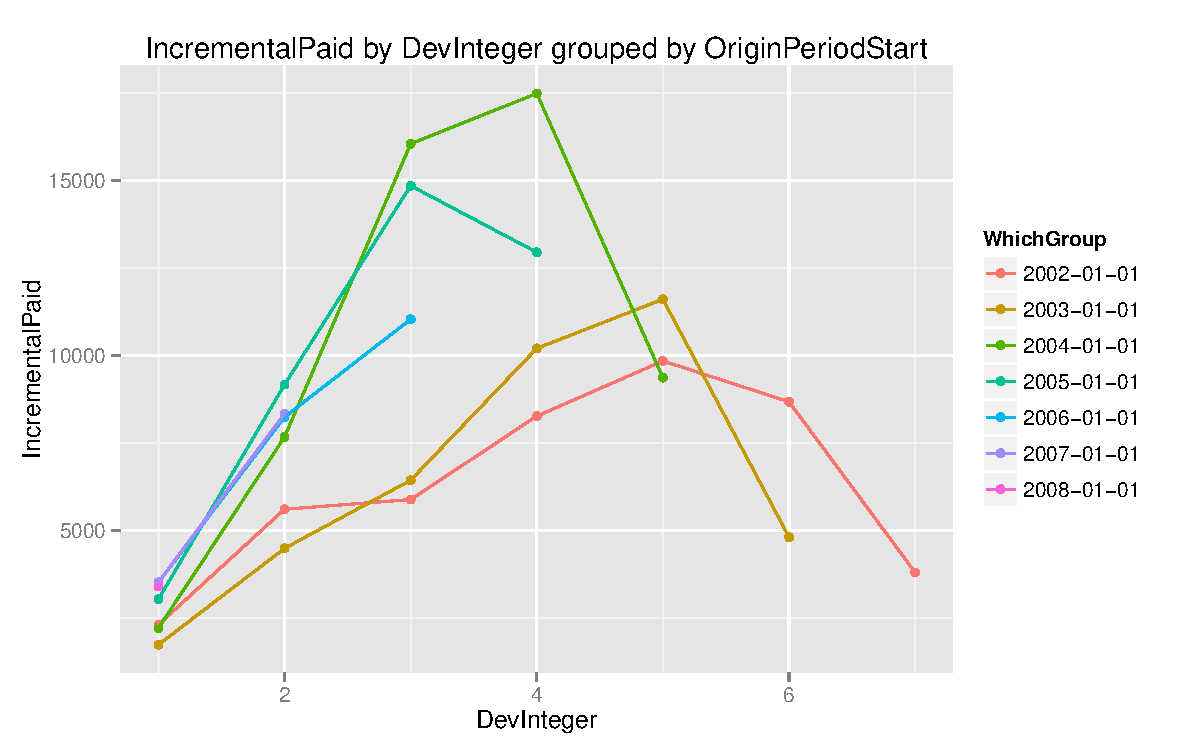
\includegraphics[width=\maxwidth]{figure/Friedland2} 

\end{knitrout}

\end{frame}

\begin{frame}[fragile]{Change the time axis}
\begin{knitrout}
\definecolor{shadecolor}{rgb}{0.969, 0.969, 0.969}\color{fgcolor}\begin{kframe}
\begin{alltt}
\hlfunctioncall{plotTriangle}(Friedland, Predictor = \hlstring{"EvaluationDate"}, 
    Response = \hlstring{"IncrementalPaid"})
\end{alltt}
\end{kframe}
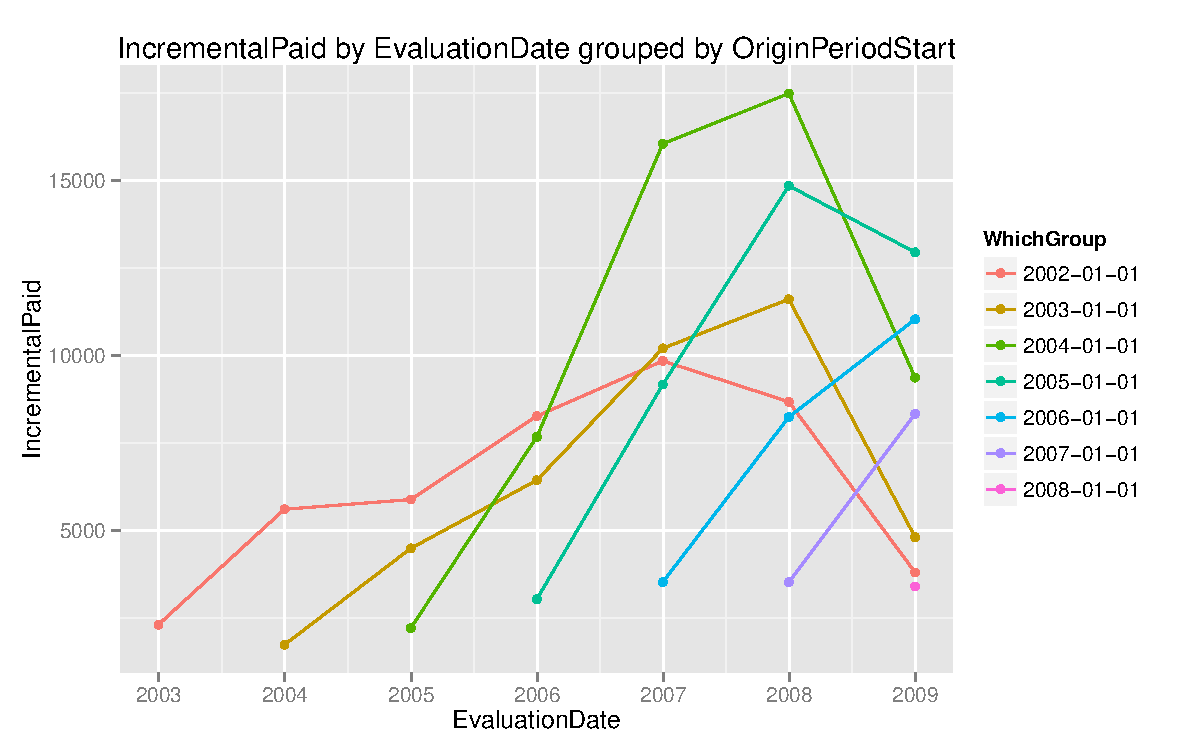
\includegraphics[width=\maxwidth]{figure/Friedland3} 

\end{knitrout}

\end{frame}

\begin{frame}[fragile]{Change the grouping dimension}
\begin{knitrout}
\definecolor{shadecolor}{rgb}{0.969, 0.969, 0.969}\color{fgcolor}\begin{kframe}
\begin{alltt}
\hlfunctioncall{plotTriangle}(Friedland, Predictor = \hlstring{"PriorPaid"}, 
    Response = \hlstring{"IncrementalPaid"}, Group = \hlstring{"DevInteger"}, 
    Lines = FALSE)
\end{alltt}


{\ttfamily\noindent\color{warningcolor}{\#\# Warning: Removed 7 rows containing missing values (geom\_point).}}\end{kframe}
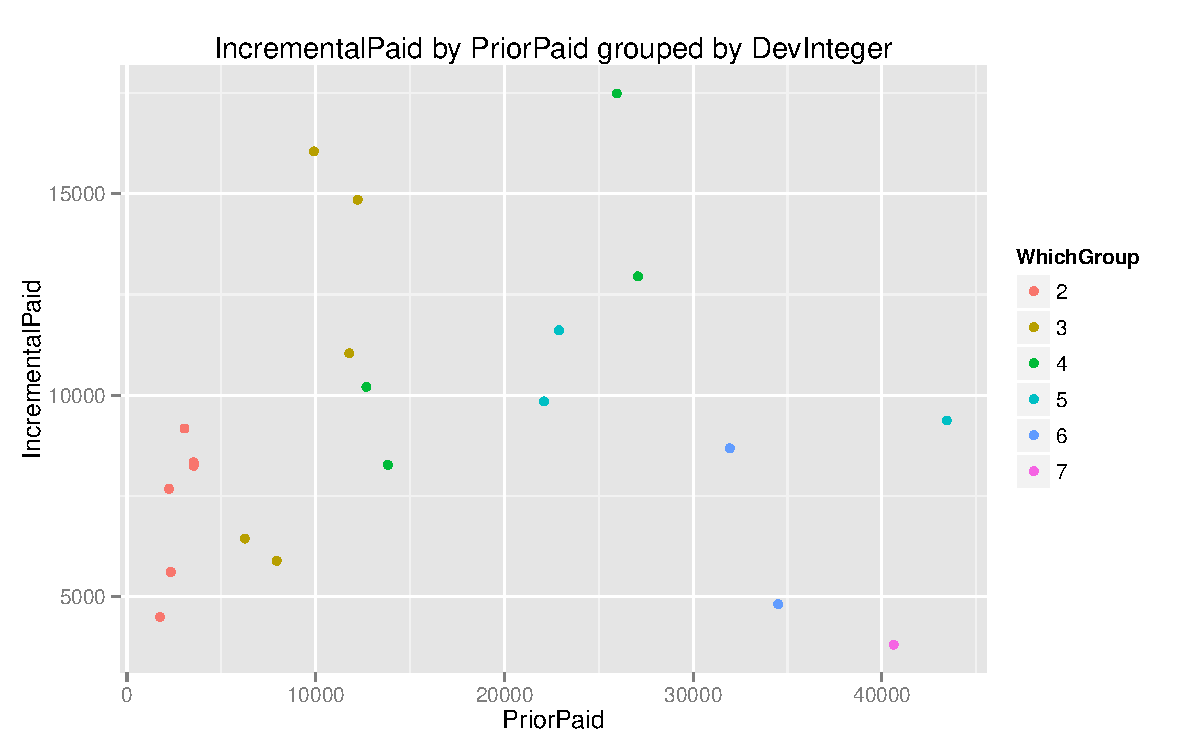
\includegraphics[width=\maxwidth]{figure/FriedlandCL1} 

\end{knitrout}

\end{frame}

\begin{frame}[fragile]{Add fit lines}
\begin{knitrout}
\definecolor{shadecolor}{rgb}{0.969, 0.969, 0.969}\color{fgcolor}\begin{kframe}
\begin{alltt}
\hlfunctioncall{plotTriangle}(Friedland, Predictor = \hlstring{"PriorPaid"}, 
    Response = \hlstring{"IncrementalPaid"}, Group = \hlstring{"DevInteger"}, 
    Lines = FALSE, FitLines = TRUE)
\end{alltt}


{\ttfamily\noindent\color{warningcolor}{\#\# Warning: Removed 7 rows containing missing values (stat\_smooth).}}

{\ttfamily\noindent\color{warningcolor}{\#\# Warning: Removed 7 rows containing missing values (geom\_point).}}\end{kframe}
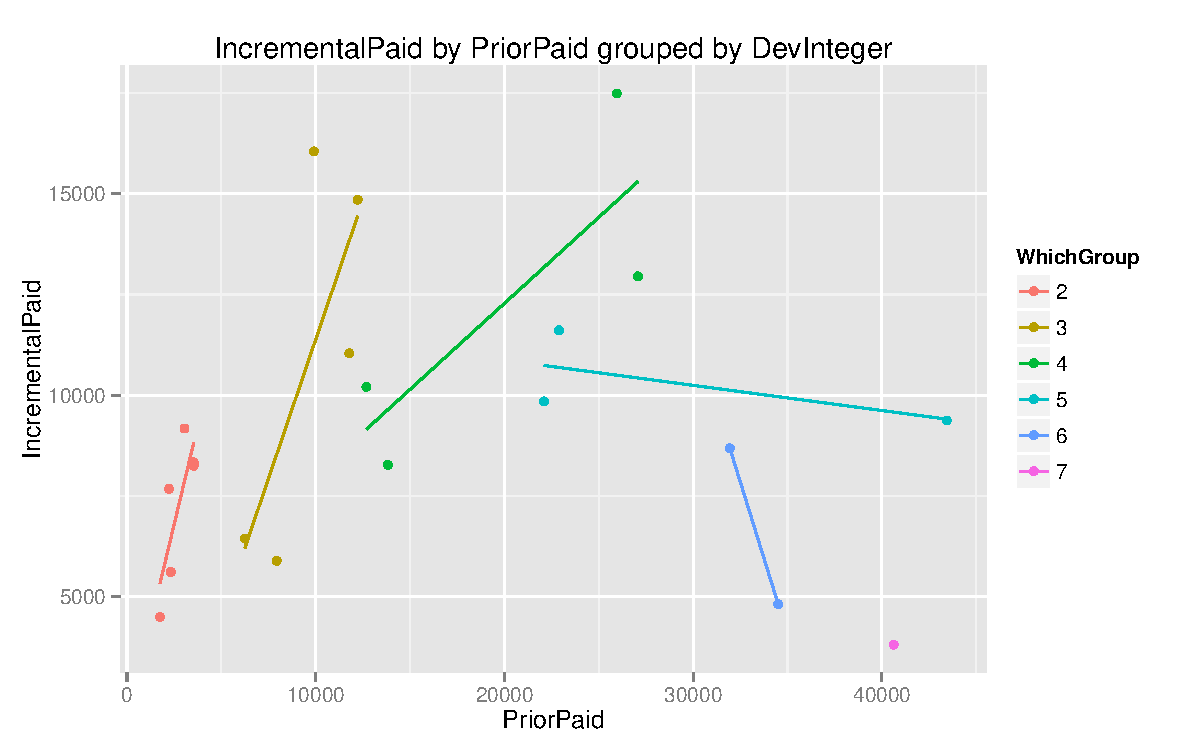
\includegraphics[width=\maxwidth]{figure/Friedland5} 

\end{knitrout}

\end{frame}

\begin{frame}[fragile]{Change the predictor variable}
\begin{knitrout}
\definecolor{shadecolor}{rgb}{0.969, 0.969, 0.969}\color{fgcolor}\begin{kframe}
\begin{alltt}
\hlfunctioncall{plotTriangle}(Friedland, Response = \hlstring{"IncrementalPaid"}, 
    Predictor = \hlstring{"EP"}, Group = \hlstring{"DevInteger"}, 
    Lines = FALSE, FitLines = TRUE)
\end{alltt}
\end{kframe}
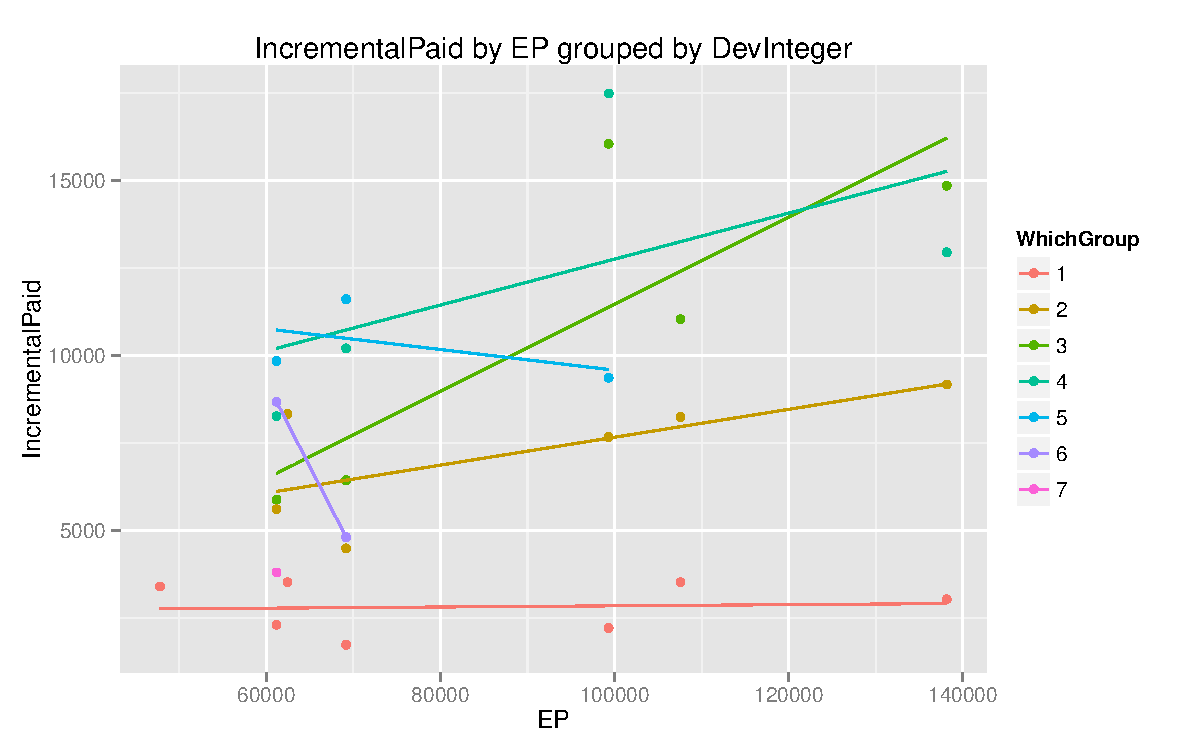
\includegraphics[width=\maxwidth]{figure/Friedland4} 

\end{knitrout}

\end{frame}

\begin{frame}[fragile]{Fit a model}
\begin{knitrout}
\definecolor{shadecolor}{rgb}{0.969, 0.969, 0.969}\color{fgcolor}\begin{kframe}
\begin{alltt}
PaidAM1 = \hlfunctioncall{newTriangleModel}(Triangle = Friedland, 
    Response = \hlstring{"IncrementalPaid"}, Predictor = \hlstring{"EP"}, 
    FitCategory = \hlstring{"DevInteger"}, Tail = 6)
\end{alltt}
\end{kframe}
\end{knitrout}

\end{frame}

\begin{frame}[fragile]{Visualization is closely related to a model}
\begin{knitrout}
\definecolor{shadecolor}{rgb}{0.969, 0.969, 0.969}\color{fgcolor}\begin{kframe}
\begin{alltt}
\hlfunctioncall{plotTriangle}(Friedland, Response = \hlstring{"IncrementalPaid"}, 
    Predictor = \hlstring{"EP"}, Group = \hlstring{"DevInteger"}, 
    Lines = FALSE, FitLines = TRUE)
PaidAM1 = \hlfunctioncall{newTriangleModel}(Friedland, Response = \hlstring{"IncrementalPaid"}, 
    Predictor = \hlstring{"EP"}, FitCategory = \hlstring{"DevInteger"}, 
    Tail = 6)
\end{alltt}
\end{kframe}
\end{knitrout}

\end{frame}

\begin{frame}[fragile]{A detour through linear regression}
\begin{knitrout}
\definecolor{shadecolor}{rgb}{0.969, 0.969, 0.969}\color{fgcolor}\begin{kframe}
\begin{alltt}
\hlfunctioncall{set.seed}(1234)
N = 100
e = \hlfunctioncall{rnorm}(N, mean = 0, sd = 1)
B0 = 5
B1 = 1.5

X1 = \hlfunctioncall{rep}(\hlfunctioncall{seq}(1, 10), 10)
Y = B0 + B1 * X1 + e

df = \hlfunctioncall{data.frame}(Y = Y, X1 = X1, e = e)
\end{alltt}
\end{kframe}
\end{knitrout}

\end{frame}

\begin{frame}[fragile]{Fitting a linear model}
\begin{knitrout}
\definecolor{shadecolor}{rgb}{0.969, 0.969, 0.969}\color{fgcolor}\begin{kframe}
\begin{alltt}
myFit = \hlfunctioncall{lm}(Y ~ X1, data = df)
\end{alltt}
\end{kframe}
\end{knitrout}

\end{frame}

\begin{frame}[fragile]{Diagnostic output}
\begin{knitrout}
\definecolor{shadecolor}{rgb}{0.969, 0.969, 0.969}\color{fgcolor}\begin{kframe}
\begin{alltt}
\hlfunctioncall{summary}(myFit)
\end{alltt}
\begin{verbatim}
## 
## Call:
## lm(formula = Y ~ X1, data = df)
## 
## Residuals:
##    Min     1Q Median     3Q    Max 
## -2.188 -0.742 -0.228  0.629  2.709 
## 
## Coefficients:
##             Estimate Std. Error t value
## (Intercept)   4.8383     0.2181    22.2
## X1            1.5009     0.0351    42.7
##             Pr(>|t|)    
## (Intercept)   <2e-16 ***
## X1            <2e-16 ***
## ---
## Signif. codes:  0 '***' 0.001 '**' 0.01 '*' 0.05 '.' 0.1 ' ' 1
## 
## Residual standard error: 1.01 on 98 degrees of freedom
## Multiple R-squared:  0.949,	Adjusted R-squared:  0.948 
## F-statistic: 1.82e+03 on 1 and 98 DF,  p-value: <2e-16
\end{verbatim}
\end{kframe}
\end{knitrout}

\end{frame}

\begin{frame}{Formulas in R}
  \begin{itemize}
    \item The '\textasciitilde' is typically read "is modeled as"
    \item The '+' operator adds new predictor variables to the model
    \item An intercept is always assumed. To remove it, add '+ 0' or '- 1' to the formula
    \item The ':' operator controls interactions between variables.
  \end{itemize}
\end{frame}

\begin{frame}[fragile]{Some examples}
\begin{knitrout}
\definecolor{shadecolor}{rgb}{0.969, 0.969, 0.969}\color{fgcolor}\begin{kframe}
\begin{alltt}
\hlcomment{# The 1 is not necessary}
\hlfunctioncall{lm}(Y ~ 1 + X1, data = df)
\hlcomment{# This is the same as above}
\hlfunctioncall{lm}(Y ~ X1, data = df)

\hlfunctioncall{lm}(Y ~ 0 + X1, data = df)  \hlcomment{#No intercept}

\hlfunctioncall{lm}(Y ~ X1 + X2, data = df)  \hlcomment{#Two predictors}

\hlcomment{# Two predictors and an interaction}
\hlfunctioncall{lm}(Y ~ X1 + X2 + X1:X2, data = df)
\end{alltt}
\end{kframe}
\end{knitrout}

\end{frame}

\begin{frame}[fragile]{Diagnostics}
\begin{knitrout}
\definecolor{shadecolor}{rgb}{0.969, 0.969, 0.969}\color{fgcolor}\begin{kframe}
\begin{alltt}
\hlfunctioncall{summary}(myFit)$r.squared
\end{alltt}
\begin{verbatim}
## [1] 0.949
\end{verbatim}
\begin{alltt}
\hlfunctioncall{summary}(myFit)$fstatistic
\end{alltt}
\begin{verbatim}
## value numdf dendf 
##  1824     1    98
\end{verbatim}
\end{kframe}
\end{knitrout}

\end{frame}

\begin{frame}[fragile]{Diagnostics pt.2}
\begin{knitrout}
\definecolor{shadecolor}{rgb}{0.969, 0.969, 0.969}\color{fgcolor}\begin{kframe}
\begin{alltt}
\hlfunctioncall{as.data.frame}(\hlfunctioncall{summary}(myFit)$coefficients)
\end{alltt}
\begin{verbatim}
##             Estimate Std. Error t value
## (Intercept)    4.838    0.21808   22.19
## X1             1.501    0.03515   42.70
##              Pr(>|t|)
## (Intercept) 5.423e-40
## X1          3.863e-65
\end{verbatim}
\end{kframe}
\end{knitrout}

\end{frame}

\begin{frame}[fragile]{Plot the data}
\begin{knitrout}
\definecolor{shadecolor}{rgb}{0.969, 0.969, 0.969}\color{fgcolor}\begin{kframe}
\begin{alltt}
\hlfunctioncall{plot}(df$X1, df$Y, pch = 19)
\hlfunctioncall{abline}(myFit$coefficients[[1]], myFit$coefficients[[2]])
\end{alltt}
\end{kframe}
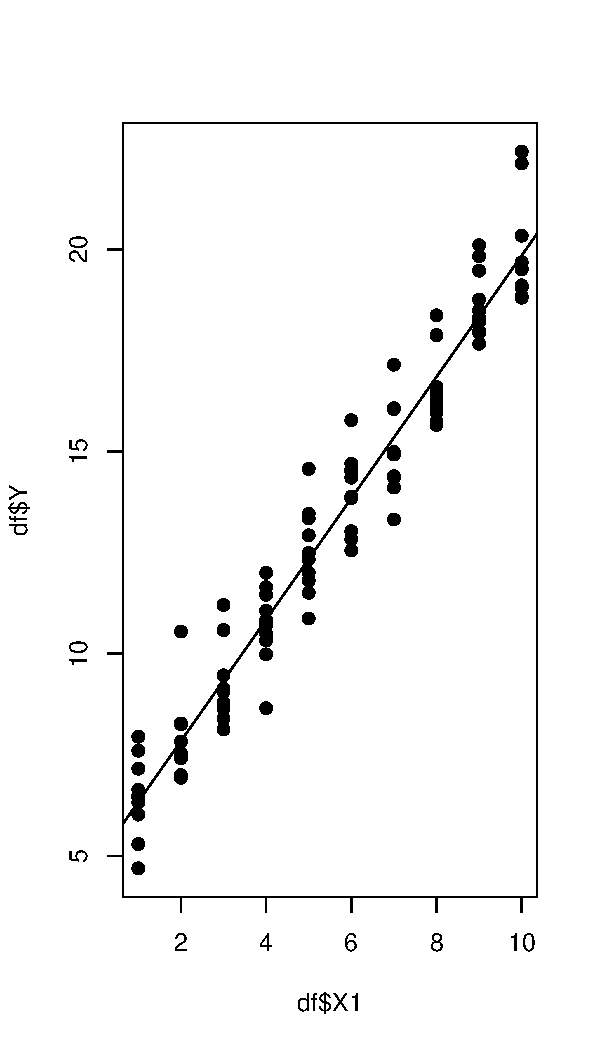
\includegraphics[width=\maxwidth]{figure/UnivariatePlot} 

\end{knitrout}

\end{frame}
\end{document}
